\documentclass[conference]{IEEEtran}
\usepackage{amsmath}
\usepackage{graphicx}
\usepackage{url}
\graphicspath{{figures/}{report/figures/}}

\title{Counting Metal Tubes and Detecting Shape Defects}
% Add any remaining group authors and affiliations before submission.
\author{\IEEEauthorblockN{Magnus Johansen}
\IEEEauthorblockA{MVCOMP01 Image Analysis}}

\begin{document}
\maketitle

\begin{abstract}
We count metal tubes and identify deformed ones in photographs using color, edges, and reflections. A foreground mask gives the first tube regions, while a distance-based heatmap combines edges and bright reflection streaks. Geometric rules merge fragments, split touching tubes, and recover tubes visible only in the edge image. The anomaly stage then checks how long and straight the reflection is inside each detected tube. Both tasks returned the correct count for every image in the supplied set of 30. The same images were used to choose thresholds, so the results describe this dataset.
\end{abstract}

\begin{IEEEkeywords}
image segmentation, object counting, reflection, anomaly detection
\end{IEEEkeywords}

\section{Introduction}
The aim is to count all metal tubes in a photograph and mark those that are deformed. Tubes may touch, and a single tube can appear as several disconnected patches after thresholding. Bright streaks help locate tubes, but they change with illumination. A deformed tube can keep a visible outline while losing the bright, straight streak typical of a regular tube.

Otsu thresholding supplies the main segmentation. It gives the initial tube regions, which we refine using bright reflections and Canny edges. Task~1 combines these cues to produce labeled tube masks and rotated bounding boxes. Task~2 uses the boxes and the original masks to examine each tube.

\section{Technical Approach}
\subsection{Preprocessing}
The opened Otsu mask is the starting point for tube segmentation. Its connected white regions give the initial tube labels. Figure~\ref{fig:otsuoverview} shows why it works well for most of the visible tubes in image 0005. Table~\ref{tab:preprocessing} summarizes the three masks.

\begin{table}[!b]
\caption{Preprocessing used in both tasks}
\label{tab:preprocessing}
\centering
\begin{tabular}{@{}p{0.21\columnwidth}p{0.72\columnwidth}@{}}
\hline
Mask & Construction and purpose \\
\hline
Foreground & Intersect inverted Otsu on HSV saturation with Otsu on Lab $a^*$. Apply rectangular $18\times18$ opening to reduce narrow background regions. \\
Reflection & Keep blue-channel values above 220. Retain 8-connected components with at least 200 pixels to obtain bright streaks. \\
Edges & Smooth HSV saturation with a $7\times7$ Gaussian filter. Apply Canny with thresholds 50 and 150 to obtain thin outlines. \\
\hline
\end{tabular}
\end{table}

Otsu chooses a threshold from the channel histogram by maximizing separation between two groups \cite{otsu}. Inverting the saturation mask selects the lower-saturation group. Intersecting it with the Lab mask adds a second color condition, which removes background pixels that pass only one test. The opening erodes and then dilates the combined mask. Features that cannot accommodate the rectangular element are removed \cite{opencvfilter}.

\begin{figure}[!ht]
\centering
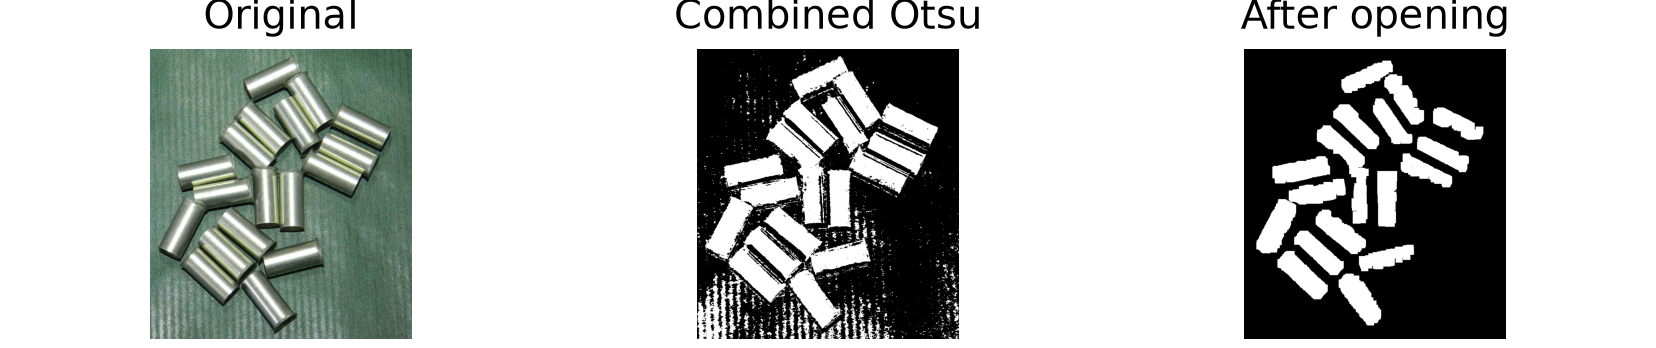
\includegraphics[width=\columnwidth]{otsu_overview_0005.png}
\caption{Main segmentation on image 0005. The combined Otsu mask captures most tube bodies. Opening removes narrow responses on the textured background and leaves the main regions used for labeling.}
\label{fig:otsuoverview}
\end{figure}

The blue-channel threshold selects bright pixels, so a blue-tinted surface can still fall below 220. A tube with a weak specular streak can be absent from the reflection mask even when its body remains visible in the color mask. Figure~\ref{fig:prep} shows where the auxiliary masks help. Canny responds to local changes in saturation after smoothing \cite{canny}. It can retain edges of dim and deformed tubes, but it also responds to the background and to details on tubes that have already been found.

\begin{figure*}[t]
\centering
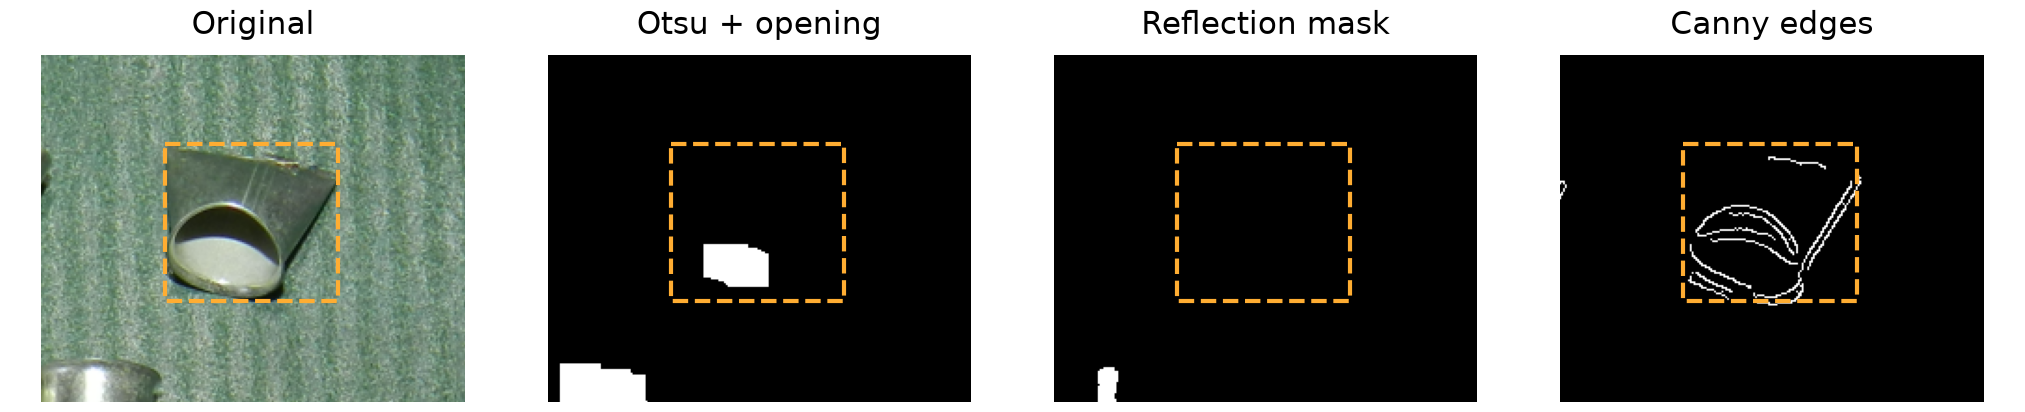
\includegraphics[width=0.71\textwidth]{preprocessing.png}
\par\vspace{0.25em}
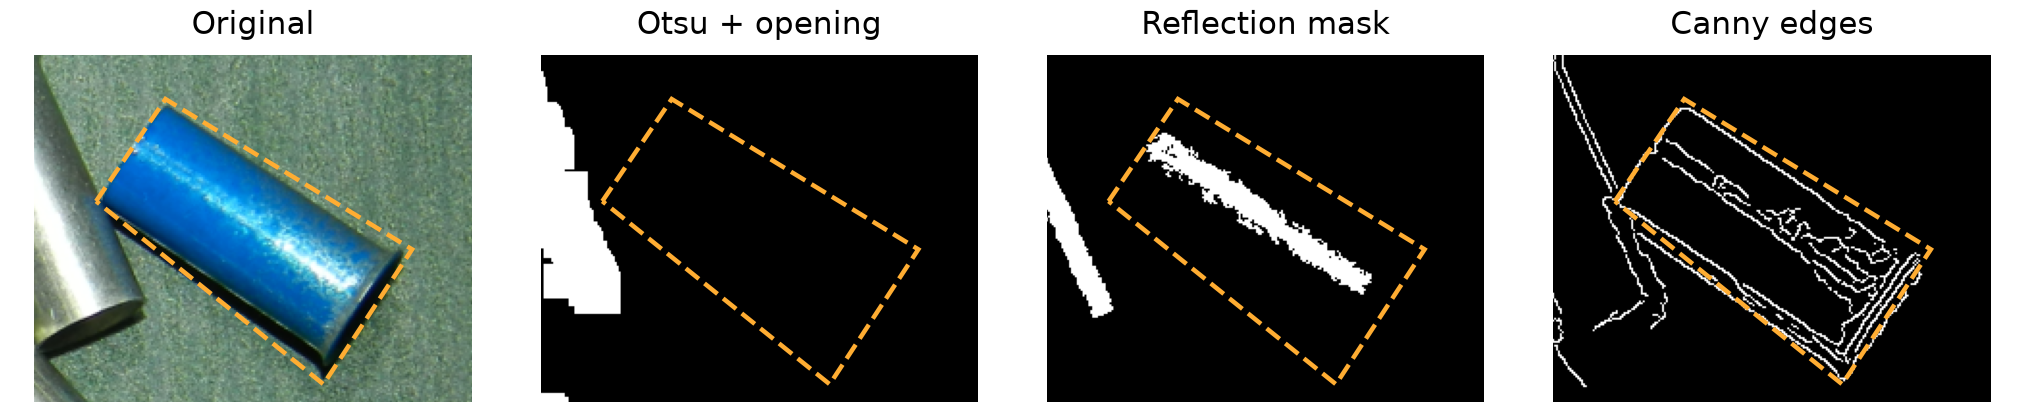
\includegraphics[width=0.71\textwidth]{blue_tube_0001.png}
\caption{Top, image 0014. The boxed deformed tube leaves a small patch in the opened mask and no retained reflection. Task~1 recovers it from Canny. Bottom, image 0001. The opened color mask misses the boxed blue tube. The reflection mask retains a bright strip, and Canny traces the outline. Task~1 retains the reflection region with heatmap support.}
\label{fig:prep}
\end{figure*}

\subsection{Counting and heatmap support}
The heatmap starts from the union $E$ of the Canny and reflection masks. For each pixel $p$, $d(p)$ is the Euclidean distance to the nearest pixel in $E$. The support is
\begin{equation}
H(p)=
\begin{cases}
\exp[-d(p)^2/(2\cdot5^2)], & d(p)\leq 10,\\
0, & d(p)>10.
\end{cases}
\end{equation}
The weight is one on an evidence pixel and about 0.61 five pixels away. This supports nearby foreground even when a thin Canny edge lies outside a cluster. Figure~\ref{fig:heatmap} shows the support across the full image.

\begin{figure}[!ht]
\centering
\begin{tabular}{@{}c@{\hspace{0.015\columnwidth}}c@{\hspace{0.015\columnwidth}}c@{}}
\scriptsize Canny + reflections & \scriptsize Heatmap overlay & \scriptsize Otsu + opening \\
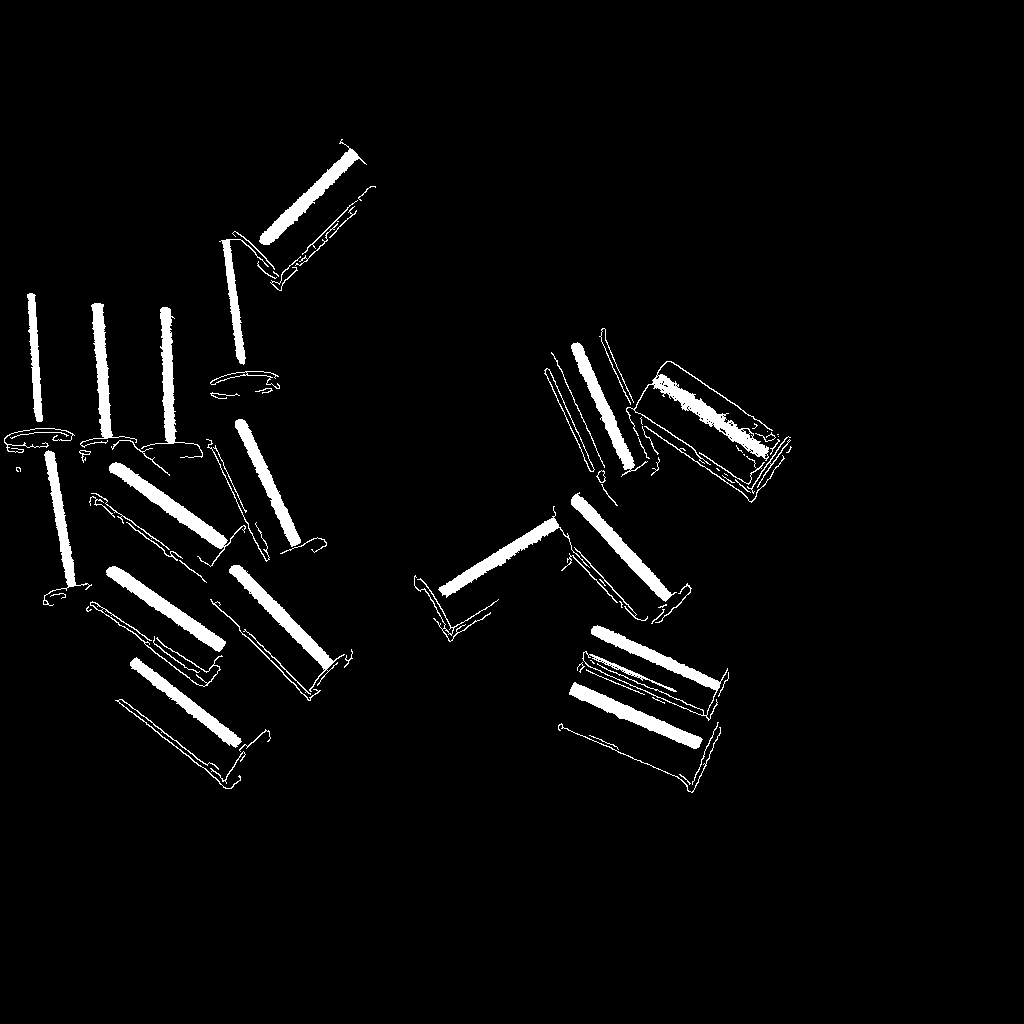
\includegraphics[width=0.32\columnwidth]{heatmap_evidence_0001.png} &
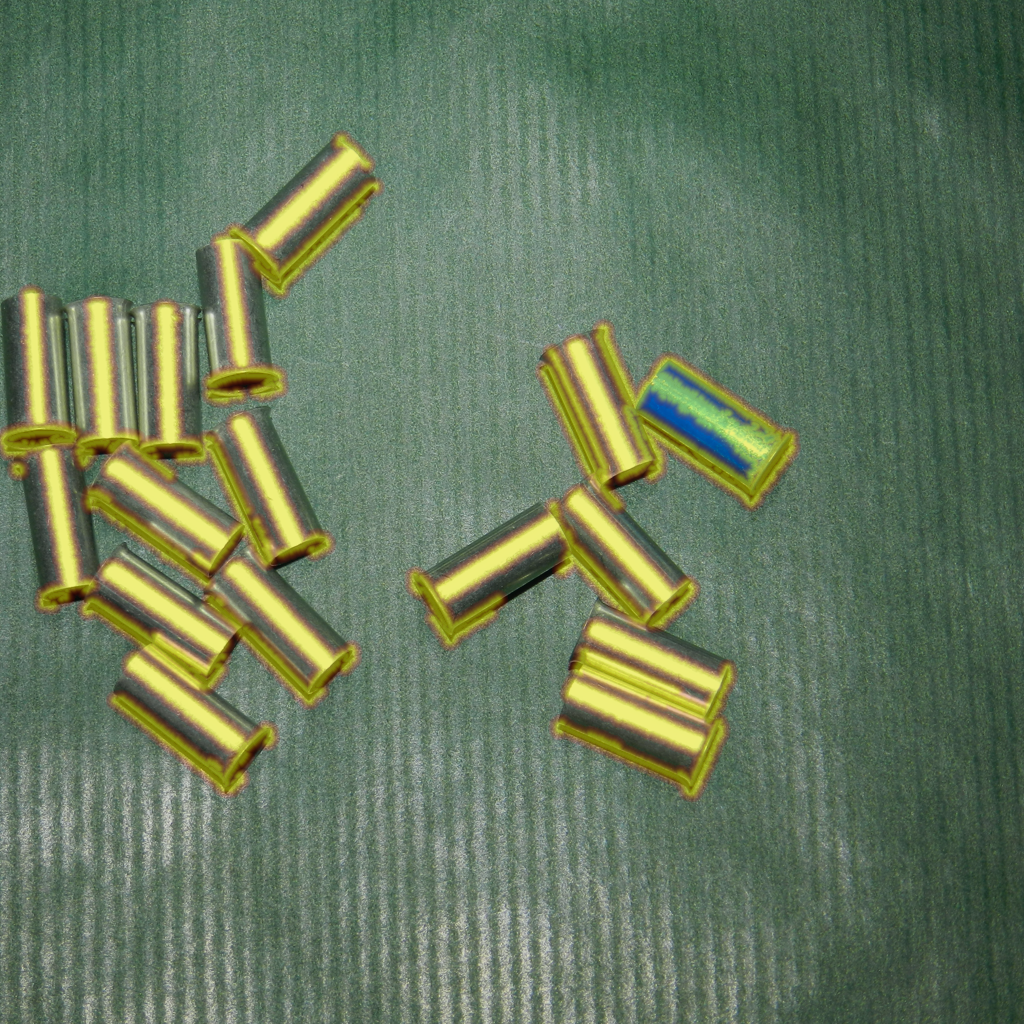
\includegraphics[width=0.32\columnwidth]{heatmap_0001.png} &
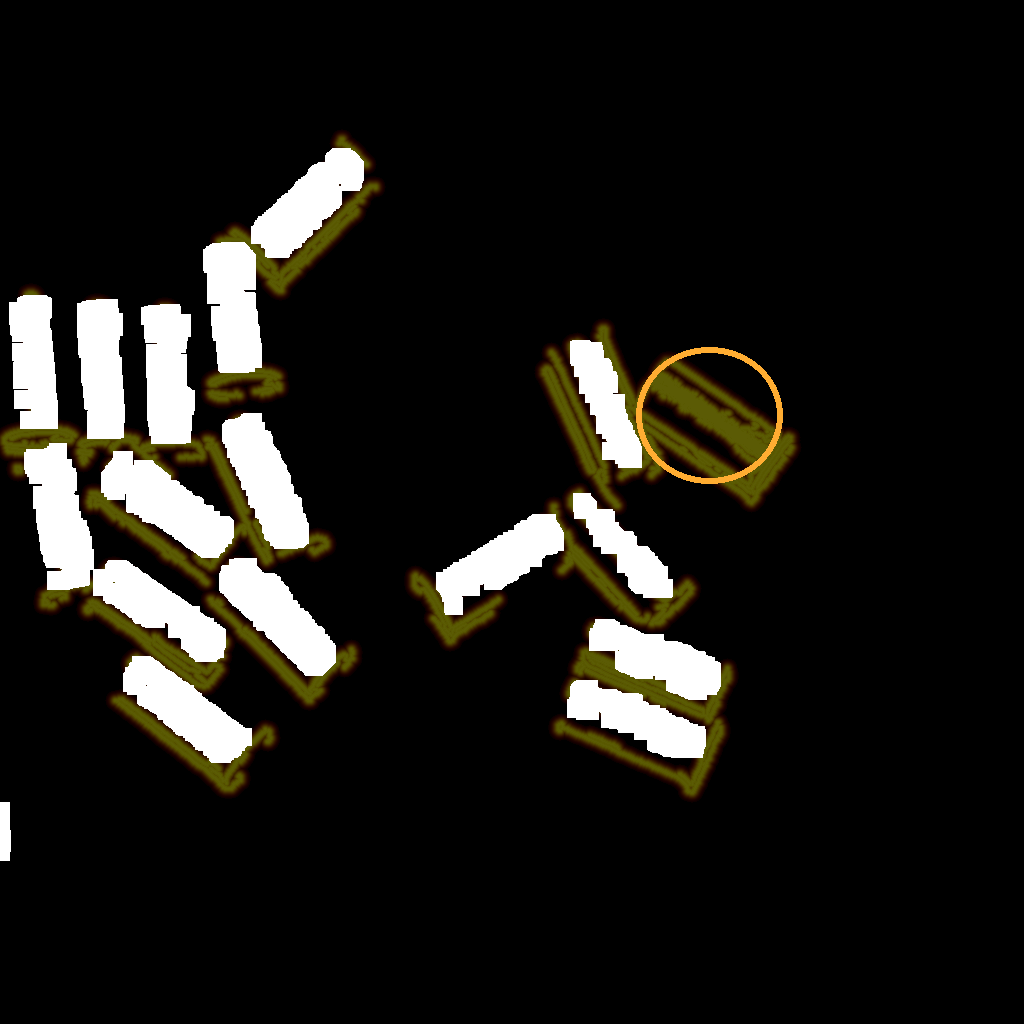
\includegraphics[width=0.32\columnwidth]{otsu_opening_0001.png}
\end{tabular}
\caption{Full image 0001. On the right, the white foreground mask sits over a faint heatmap. The ring shows heatmap support at the blue tube, where the foreground mask is empty.}
\label{fig:heatmap}
\end{figure}

The initial clusters are the 8-connected components of the opened color mask. Adding the reflection mask can extend a cluster or contribute a new candidate. If a combined region contains multiple original clusters, their labels remain separate at this stage. A bright streak can connect adjacent but distinct tubes.

A cluster is kept if its mean heatmap support is at least 0.15 or if it has a strong tube shape. The shape test requires at least 2,200 pixels, a long side of at least 85 pixels, a short side of at least 18 pixels, an aspect ratio of at least 2.5, and at least 55\% fill of the rotated bounding box. The aspect ratio may fall to 2.2 if at least 20\% of the cluster lies within eight pixels of positive heatmap support. Weak neighboring fragments are checked again after merging, so together they can provide enough shape evidence.

In a development run on image 0029, the $20\times20$ opening left background fragments that appeared tube-shaped after merging. The length rule split that region into two false detections. With the $18\times18$ opening, the merged region filled less of its bounding box and was wider relative to its length. The shape filter rejected it before splitting.



\subsection{Merging fragments of the same tube}
Illumination can break a tube into separate patches. If a reflection at least 45 pixels long overlaps multiple clusters, fragments under 800 pixels may join the largest cluster along that streak. Nearby fragments under 2,000 pixels may also join a neighbor within 16 pixels. Small regions without streak support are removed. In Fig.~\ref{fig:merge}, three patches receive the same label and count as one tube.

\begin{figure}[!ht]
\centering
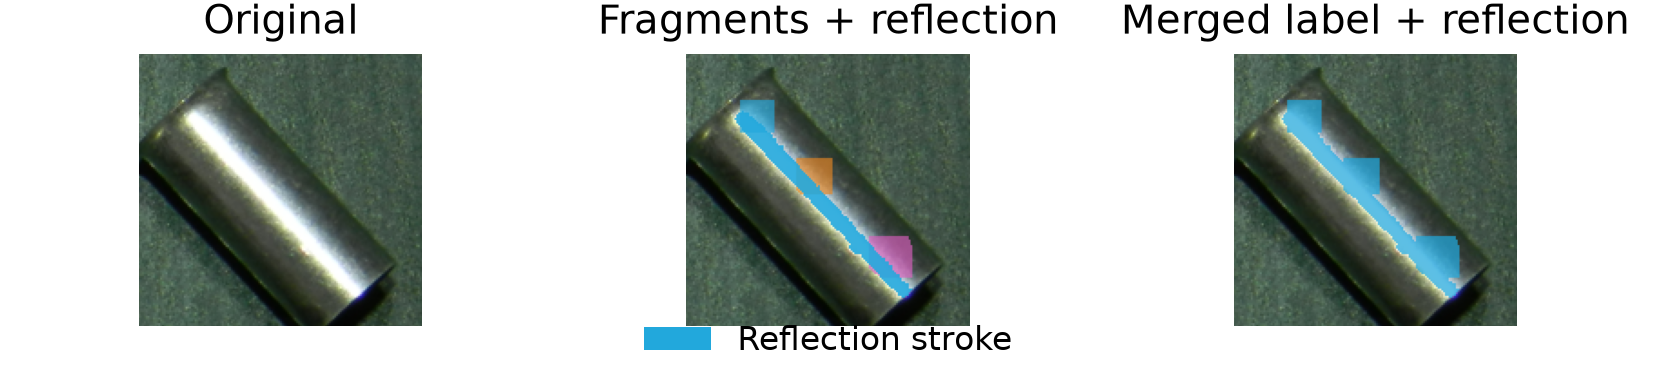
\includegraphics[width=\columnwidth]{edge_merge_0003.png}
\caption{Image 0003. The blue reflection runs through all three colored fragments in the middle. On the right, the reflection and the shared label are shown in blue. The label assignment itself leaves the gaps unchanged.}
\label{fig:merge}
\end{figure}

\subsection{Splitting a cluster using reflection strokes}
The function \texttt{split\_clusters\_by\_strokes} asks whether a cluster contains evidence of distinct tube axes. It crops to the cluster and retains only reflection pixels inside it. An orthogonal line fit gives a unit direction $\mathbf v$ for each reflection component. The pixels are projected onto $\mathbf v$ and their span must be at least 75 pixels. If fewer than two candidates are found, a local probabilistic Hough search proposes straight segments \cite{hough,opencvfilter}. This can recover separate directions when touching reflections share one component label.

For two directions, the undirected angle is
\begin{equation}
\alpha=\arccos\!\left(\lvert\mathbf v_1^\top\mathbf v_2\rvert\right).
\end{equation}
An angle of at least $25^\circ$ provides evidence of separate axes. The absolute value treats opposite directions along the same axis as equivalent. Nearly parallel strokes can still belong to different tubes. In that case, at least 80\% of each stroke must lie in the cluster, their perpendicular separation must be at least 30 pixels, and the overlap along the axes must be at least 45\% of the shorter projected span. A cluster with aspect ratio at most two and at least 80\% rectangular fill is protected from this split. A single crushed tube can have reflections pointing in several directions.

For retained stroke masks $S_j$, each cluster pixel $p$ is assigned to the nearest actual stroke pixel:
\begin{equation}
j^*(p)=\arg\min_j\;\min_{q\in S_j}\lVert p-q\rVert_2.
\end{equation}
Proposed parts under 200 pixels are discarded as split candidates. If at least two parts remain, the original pixels are reassigned among the retained strokes and each part gets its own label. Figure~\ref{fig:splitgeometry} illustrates the assignment, and Fig.~\ref{fig:split} shows the result on image 0024.

\begin{figure}[!ht]
\centering
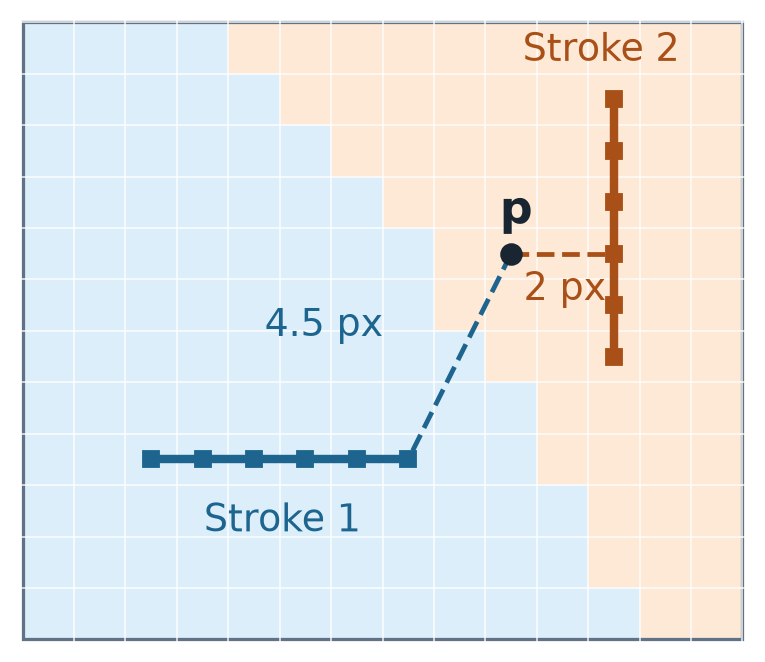
\includegraphics[width=0.77\columnwidth]{stroke_split_geometry.png}
\caption{Schematic split on a pixel grid. The two stroke directions differ by $90^\circ$, above the $25^\circ$ threshold. Blue and orange cells show the closest stroke. Pixel $p$ is closer to stroke 2 and takes its label. Dashed lines connect $p$ to the closest recorded pixel on each stroke.}
\label{fig:splitgeometry}
\end{figure}

\begin{figure}[!ht]
\centering
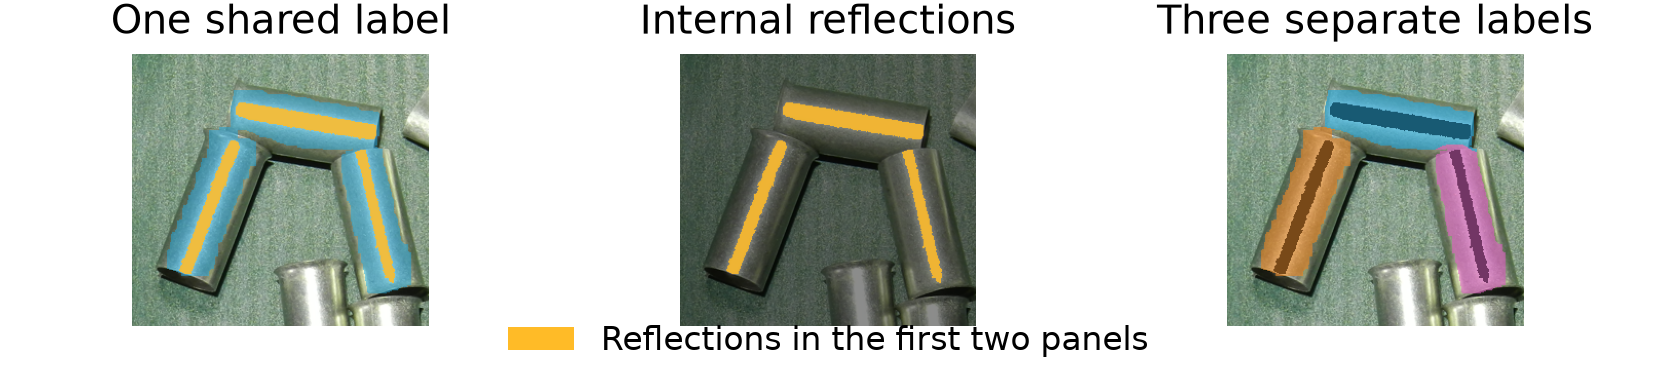
\includegraphics[width=0.87\columnwidth]{stroke_split.png}
\caption{Image 0024. Gold shows the internal reflections in the first two panels. On the right, each reflection is a darker shade of the label it helps define.}
\label{fig:split}
\end{figure}

\subsection{Splitting an unusually long cluster}
End-to-end tubes can form a single long region. A separate rule splits a cluster at its midpoint along its long axis if its length is at least 30\% above the image mean. In Fig.~\ref{fig:length}, the cluster measures 283 pixels against a cutoff of about 203 pixels.

\begin{figure}[!ht]
\centering
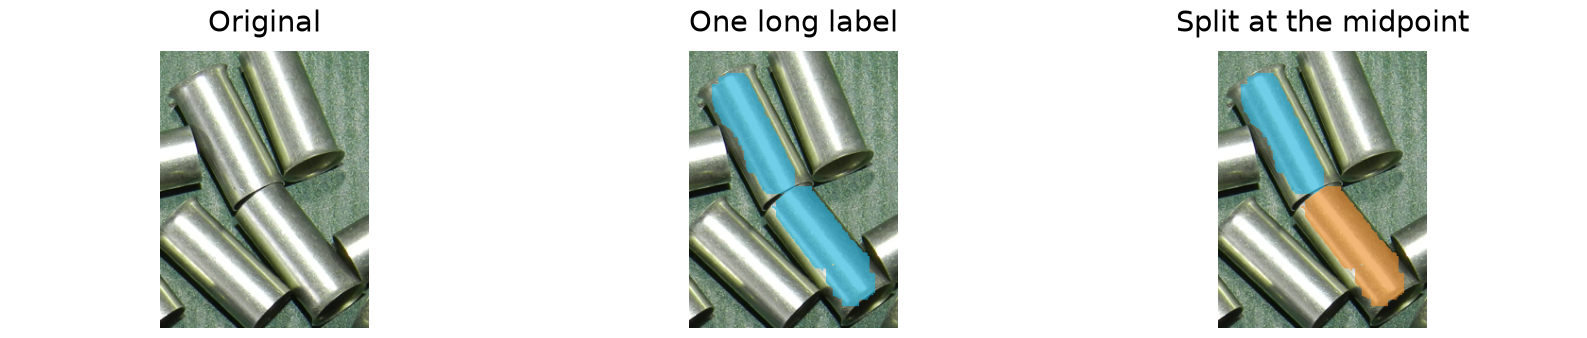
\includegraphics[width=\columnwidth]{edge_length_0007.png}
\caption{Image 0007. Two end-to-end tubes share one long label. The midpoint split gives the two halves separate labels near the join.}
\label{fig:length}
\end{figure}

\subsection{Recovering missed tubes with Canny}
We thicken Canny and close gaps using $9\times9$ elliptical elements. An entire connected edge region is discarded if it touches a tube label. The remaining regions are checked for area (750--8,500 pixels), short side ($\geq25$ pixels), long side ($\leq165$ pixels), and aspect ratio ($\leq2$). An accepted region adds one tube and carries a Canny-only flag into Task~2. In Fig.~\ref{fig:cannyrecovery}, the box contains no retained reflection. The saturation change still produces a Canny outline. The thickened edge region has 1,059 pixels, sides of about 50 and 54 pixels, and zero overlap with earlier labels. It passes the geometry checks, which use Canny alone at this stage.

\begin{figure}[!ht]
\centering
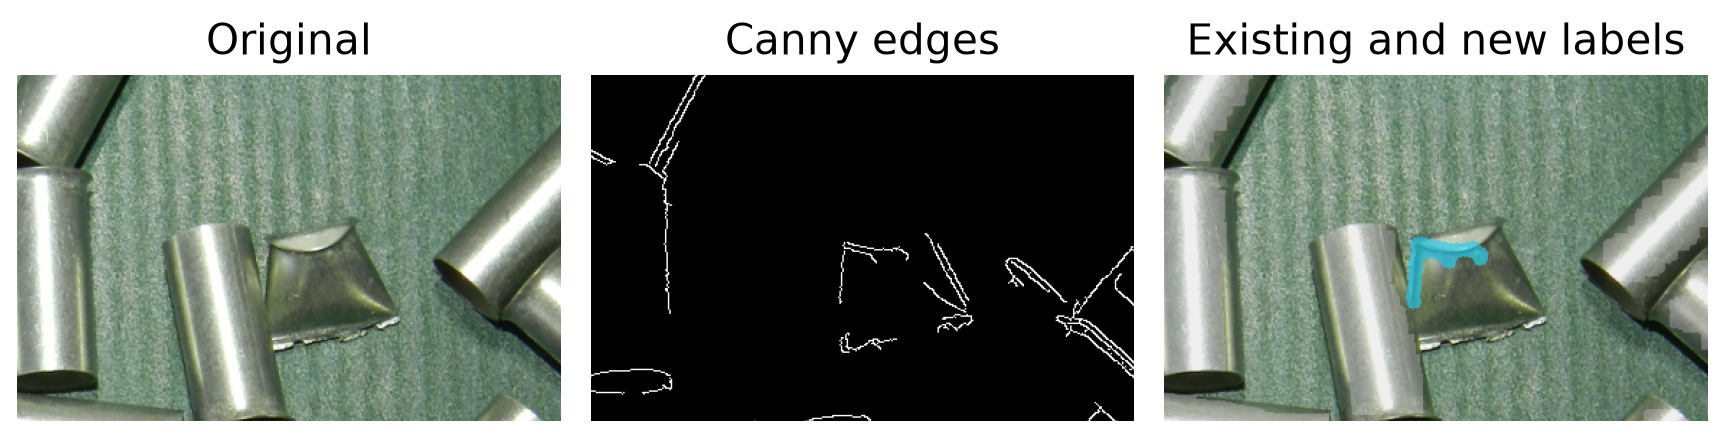
\includegraphics[width=\columnwidth]{edge_canny_0009.png}
\caption{Image 0009. Cyan identifies the newly accepted Canny region among the neighboring tubes. Gray shows earlier labels.}
\label{fig:cannyrecovery}
\end{figure}

Each final tube label is represented by a minimum-area rotated bounding box and the mean position of its pixels.

\subsection{Detecting anomalies}
Task~2 clips the reflection mask to each rotated tube box. If the largest connected reflection has at least twice as many pixels as all others combined, only that component is measured. This avoids giving a few pixels from a neighboring tube the same weight as the main streak.

We use \texttt{fitLine} with $L_2$ distance to fit an axis to the selected pixels \cite{opencvshape}. For a pixel $\mathbf p_i=(x_i,y_i)^\top$, let $\mathbf p_0$ be a point on the fitted line and $\mathbf v=(v_x,v_y)^\top$ its unit direction. The signed perpendicular distance and its population standard deviation are
\begin{align}
d_i &= (\mathbf p_i-\mathbf p_0)^\top(-v_y,v_x)^\top,\\
s_d &= \sqrt{\frac{1}{n}\sum_{i=1}^{n}(d_i-\bar d)^2}.
\end{align}
The $L_2$ fit minimizes the sum of squared perpendicular distances. It works at any orientation, including nearly vertical tubes. A bent reflection can spread far from its best-fit line even when its bounding box is long. Thickness can also increase $s_d$, so the threshold of eight pixels is an empirical rule. In Fig.~\ref{fig:fit}, the deformed tube gives $s_d=8.75$ pixels.

A tube is flagged if it came from Canny alone, contains no pixels of the opened mask, or has $s_d>8$. For the remaining tubes we measure reflection length as the long side of its minimum-area rectangle. A reflection at or below $0.70L_{\max}$, where $L_{\max}$ is the longest measured reflection in that image, triggers a final check. The tube is kept as normal if its cluster box exceeds that limit and is at least 2.5 times as long as it is wide. This protects long, narrow tubes with faint or partial reflections.

\begin{figure}[t]
\centering
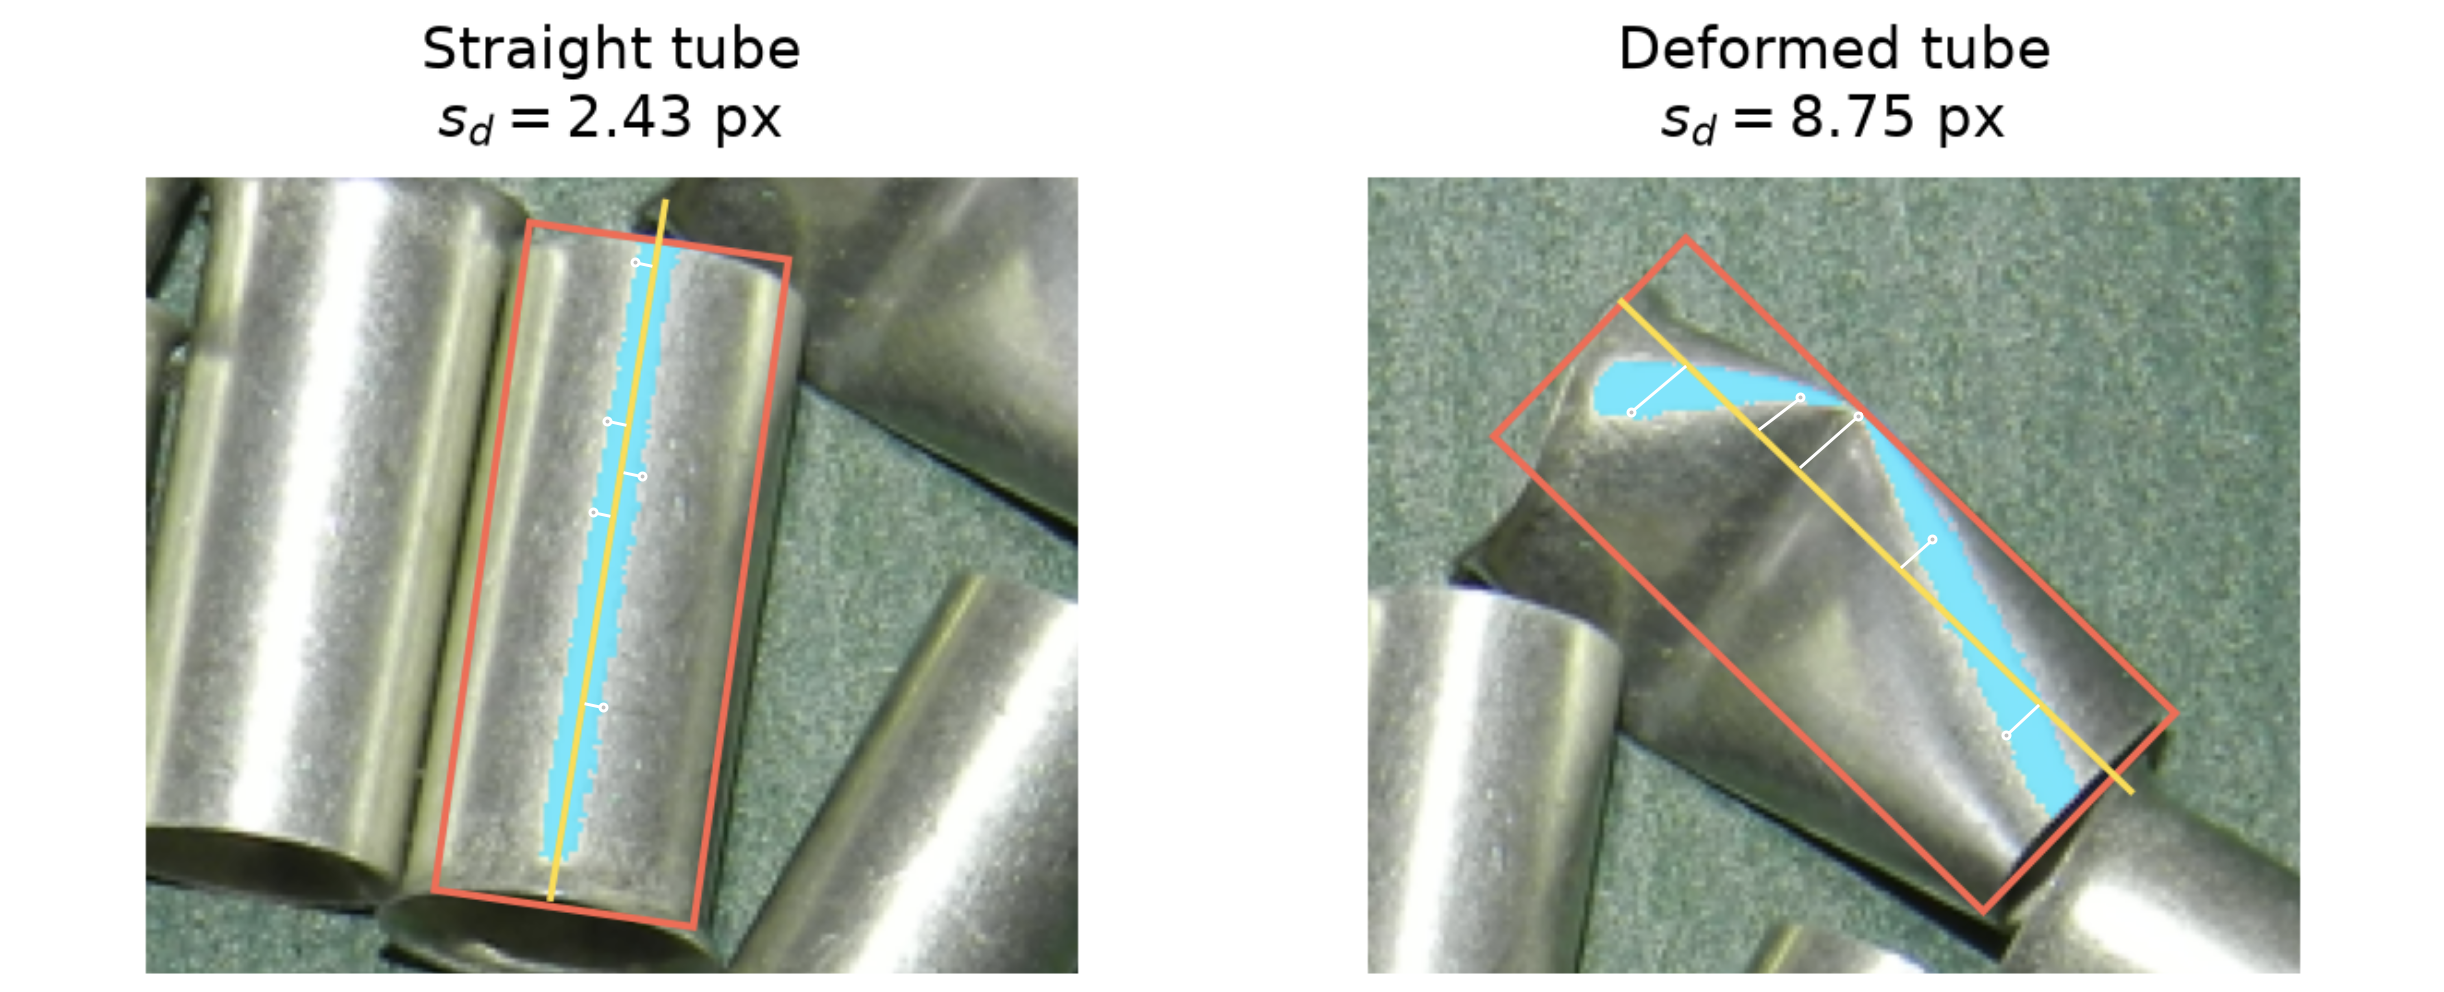
\includegraphics[width=0.87\columnwidth]{reflection_fit.png}
\par\smallskip
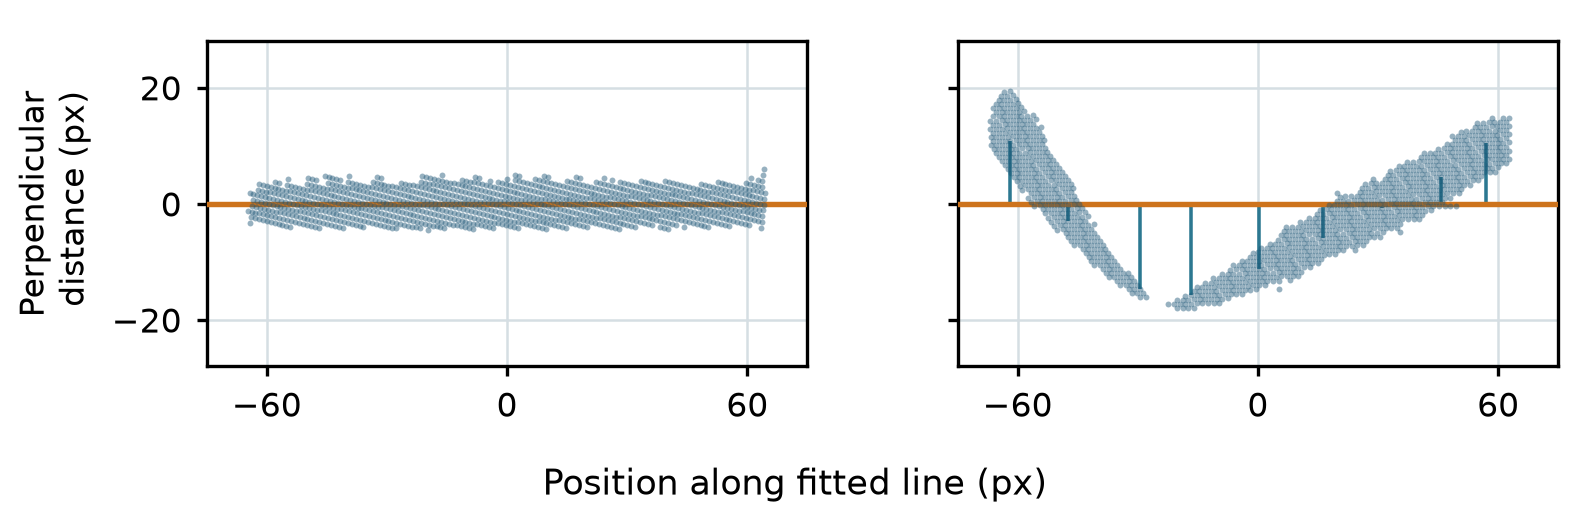
\includegraphics[width=0.98\columnwidth]{reflection_fit_residuals.png}
\caption{Image 0026. The straight tube is on the left and the deformed tube on the right. The lower plots show the same reflection pixels in coordinates aligned with each fitted line. The orange line marks zero distance. Blue segments show selected perpendicular distances. Both plots use the same scale.}
\label{fig:fit}
\end{figure}

\section{Results}
We evaluated exact counts on 30 annotated images, using the tube counts for Task~1 and the number of defect boxes for Task~2. All 24 anomaly centers fell inside distinct reference boxes.

\begin{table}[t]
\caption{Evaluation on the supplied 30 images}
\label{tab:results}
\centering
\begin{tabular}{@{}lrrr@{}}
\hline
Task & Exact images & Total found & Error SD \\
\hline
Tube counting & 30/30 & 456 & 0.00 \\
Anomaly counting & 30/30 & 24 & 0.00 \\
\hline
\end{tabular}
\end{table}

See Table~\ref{tab:results} for counts and error spread.

\begin{table}[!t]
\caption{Effect of removing individual steps}
\label{tab:ablation}
\centering
\begin{tabular}{@{}p{0.72\columnwidth}r@{}}
\hline
Variant & Exact images \\
\hline
Task 1 without stroke-based splitting & 26/30 \\
Task 1 without Canny-only additions & 26/30 \\
Task 2 without perpendicular spread & 25/30 \\
\hline
\end{tabular}
\end{table}

Table~\ref{tab:ablation} shows the effect of removing one step at a time. Without stroke splitting, four images undercount by one, including 0024. Without Canny recovery, images 0009, 0014, 0019, and 0021 each miss one tube. The perpendicular-spread check affects five images, including 0026. Thresholds were chosen on this image set.

\newpage
\section{Conclusion}
The color mask supplies tube regions, while reflections and Canny provide the evidence needed when tubes touch or are missed. Measuring the spread around a fitted line detects bends that a length check alone misses. Both tasks achieved exact counts on the supplied images. Several thresholds, kernel sizes, and geometric rules were tuned by hand on the 30 available images. This can lead to overfitting. With so few images and no independent test set, the measured accuracy is an uncertain estimate of performance on new data. A larger, more varied dataset could contain lighting changes, background reflections, and tube arrangements that the current rules do not cover.

One improvement would be to estimate the average size of reliably detected tubes in each image. Length and area limits could then be set relative to that estimate, making them less sensitive to image scale. An independent, more diverse test set would show how well such a change generalizes.



\begin{thebibliography}{00}
\bibitem{otsu}
N. Otsu, A threshold selection method from gray-level histograms, \emph{IEEE Trans. Syst., Man, Cybern.}, vol. 9, no. 1, pp. 62--66, 1979, doi: 10.1109/TSMC.1979.4310076.
\bibitem{canny}
J. Canny, A computational approach to edge detection, \emph{IEEE Trans. Pattern Anal. Mach. Intell.}, vol. PAMI-8, no. 6, pp. 679--698, 1986, doi: 10.1109/TPAMI.1986.4767851.
\bibitem{opencvfilter}
OpenCV, Image processing, \emph{OpenCV 4.x Documentation}. [Online]. Available: \url{https://docs.opencv.org/4.x/d7/dbd/group__imgproc.html}
\bibitem{hough}
R. O. Duda and P. E. Hart, Use of the Hough transformation to detect lines and curves in pictures, \emph{Commun. ACM}, vol. 15, no. 1, pp. 11--15, 1972, doi: 10.1145/361237.361242.
\bibitem{opencvshape}
OpenCV, Structural analysis and shape descriptors, \emph{OpenCV 4.x Documentation}. [Online]. Available: \url{https://docs.opencv.org/4.x/d3/dc0/group__imgproc__shape.html}
\end{thebibliography}

\end{document}
